\begin{figure}[htbp]
\centering
% Curves: VF-FRO-10, f/a_lambda=(1-xi)[ln(mu^2/Delta)-1+(m_q+xi m_p)^2/Delta],
% Delta=xi m_s^2+(1-xi)m_q^2-xi(1-xi)m_p^2, m_q=0.3, m_p=1.0, m_s=1.5 GeV (starter code of
% FIGURES_INDEX_v2 N17; ymin/ymax widened so that no curve is clipped: f(0.001;2.5)=4.22).
% Zeros: mu=0.8: xi=0.26403; mu=1.2: xi=0.56737 (mpmath findroot); mu=2.5: min f=7.7e-4>0.
% Minimum of the mu=0.8 curve: -0.351 at xi=0.58 (labels of the zeros placed below it).
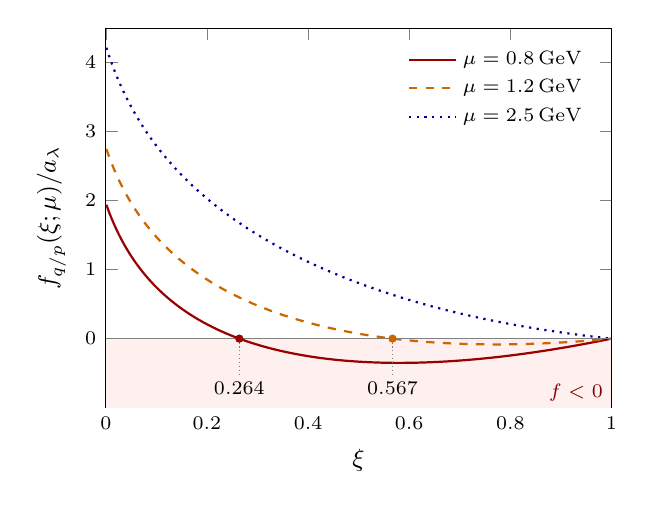
\begin{tikzpicture}
\begin{axis}[width=0.66\textwidth,height=6.4cm,xmin=0,xmax=1,ymin=-1.0,ymax=4.5,
  xlabel={$\xi$},ylabel={$f^{\MSbar}_{q/p}(\xi;\mu)/a_\lambda$},
  xtick={0,0.2,0.4,0.6,0.8,1},ytick={0,1,2,3,4},
  tick label style={font=\scriptsize},label style={font=\small},
  legend style={font=\scriptsize,draw=none,fill=none,at={(0.97,0.97)},anchor=north east},
  legend cell align=left]
\fill[red!6] (axis cs:0,-1.0) rectangle (axis cs:1,0);
\addplot[domain=0.001:0.999,samples=200,thick,red!60!black]{(1-x)*(ln(0.8^2/(2.25*x+0.09*(1-x)-x*(1-x)))-1+(0.3+x)^2/(2.25*x+0.09*(1-x)-x*(1-x)))};
\addlegendentry{$\mu=0.8\,\mathrm{GeV}$}
\addplot[domain=0.001:0.999,samples=200,thick,dashed,orange!80!black]{(1-x)*(ln(1.2^2/(2.25*x+0.09*(1-x)-x*(1-x)))-1+(0.3+x)^2/(2.25*x+0.09*(1-x)-x*(1-x)))};
\addlegendentry{$\mu=1.2\,\mathrm{GeV}$}
\addplot[domain=0.001:0.999,samples=200,thick,dotted,blue!60!black]{(1-x)*(ln(2.5^2/(2.25*x+0.09*(1-x)-x*(1-x)))-1+(0.3+x)^2/(2.25*x+0.09*(1-x)-x*(1-x)))};
\addlegendentry{$\mu=2.5\,\mathrm{GeV}$}
\draw[gray,thin] (axis cs:0,0) -- (axis cs:1,0);
\draw[gray,densely dotted] (axis cs:0.264,0) -- (axis cs:0.264,-0.56);
\draw[gray,densely dotted] (axis cs:0.567,0) -- (axis cs:0.567,-0.56);
\fill[red!60!black] (axis cs:0.264,0) circle[radius=1.5pt];
\fill[orange!80!black] (axis cs:0.567,0) circle[radius=1.5pt];
\node[font=\scriptsize,anchor=north,inner sep=1.5pt] at (axis cs:0.264,-0.56) {$0.264$};
\node[font=\scriptsize,anchor=north,inner sep=1.5pt] at (axis cs:0.567,-0.56) {$0.567$};
\node[font=\scriptsize,text=red!50!black,anchor=south east,inner sep=2pt] at (axis cs:0.995,-1.0) {$f<0$};
\end{axis}
\end{tikzpicture}
\caption{Yukawa 模型中单圈 $\MSbar$ “夸克在核子中”的分布（$m_q=0.3\,\mathrm{GeV}$、$m_p=1.0\,\mathrm{GeV}$、$m_s=1.5\,\mathrm{GeV}$，纵轴以 $a_\lambda=\lambda^2/(16\pi^2)$ 为单位）\cite{CollinsRogersSato2022}：$\mu=0.8\,\mathrm{GeV}$ 时 $\xi>0.264$ 处为负，$\mu=1.2\,\mathrm{GeV}$ 时 $\xi>0.567$ 处为负，$\mu=2.5\,\mathrm{GeV}$ 时处处为正（曲线由 VF-FRO-10 的单圈公式计算）。
“$\MSbar$ 分布在所有标度上非负”因而不成立；足够大标度上的正定性只有部分论证（\cref{prop:front-positivity-large-scale}），一般陈述仍是猜想（\cref{conj:pdf-positivity}）。}
\label{fig:front-yukawa-pdf}
\end{figure}
